\documentclass[aps,pra,showpacs,notitlepage,onecolumn,superscriptaddress,nofootinbib]{revtex4-1}
\usepackage[utf8]{inputenc}
\usepackage[tmargin=1in, bmargin=1.25in, lmargin=1.5in, rmargin=1.5in]{geometry}
\usepackage{amsmath, amssymb, amsthm}
\usepackage{graphicx}
\usepackage{xcolor}
\usepackage{enumitem}
\usepackage{datetime}
\usepackage{hyperref}
\usepackage{titlesec}
\usepackage{import}
\usepackage{mathtools}
\usepackage{thmtools,thm-restate}
\usepackage{comment}
\usepackage{tikz-cd}


% package for commutative diagrams
% \usepackage{tikz-cd}

%%%%%%%%%%%%%%%%%%%%%%%%%%%%%%%%%%%%%%%%%%%%%
\definecolor{crimson}{RGB}{186,0,44}
\definecolor{moss}{RGB}{0, 186, 111}
\newcommand{\pop}[1]{\textcolor{crimson}{#1}}
\newcommand{\zcom}[1]{\noindent\textcolor{crimson}{(Z): #1}}
\newcommand{\jcom}[1]{\noindent\textcolor{moss}{(J): #1}}
\newcommand{\wt}[1]{\widetilde{#1}}
\newcommand{\pqeq}{\succcurlyeq}
\newcommand{\pleq}{\preccurlyeq}
\newcommand{\Wedge}{\bigwedge}

%%%%%%%%%%%%%%%%%%%%%%%%%%%%%%%%%%%%%%%%%%%%%
\hypersetup{
    colorlinks,
    linkcolor={crimson},
    citecolor={crimson},
    urlcolor={crimson}
}

\usepackage{qcircuit}

%%%%%%%%%%%%%%%%%%%%%%%%%%%%%%%%%%%%%%%%%%%%%
\theoremstyle{definition}
\newtheorem{definition}{Definition}[section]
\newtheorem{lemma}{Lemma}[section]
\newtheorem{theorem}{Theorem}[section]
\newtheorem{corollary}{Corollary}[theorem]
\newtheorem*{theorem*}{Theorem}
\newtheorem*{corollary*}{Corollary}
\newtheorem{remark}{Remark}[section]
\newtheorem{conjecture}{Conjecture}[section]
\newtheorem{example}{Example}[section]
\newtheorem{reminder}{Reminder}[section]
\newtheorem{problem}{Problem}[section]
\newtheorem{question}{Question}[section]
\newtheorem{answer}{Answer}[section]
\newtheorem{fact}{Fact}[section]
\newtheorem{claim}{Claim}[section]

\newcommand{\hhrulefill}{\hspace{-1.5em} \hrulefill}

\usepackage{geometry}
\geometry{
  left=25mm,
  right=25mm,
  top=20mm,
}

%%%%%%%%%%%%%%%%%%%%%%%%%%%%%%%%%%%%%%%%%%%%%
\bibliographystyle{unsrt}

%%%%%%%%%%%%%%%%%%%%%%%%%%%%%%%%%%%%%%%%%%%%%
%%%%%%%%%%%%%%%%%%%%%%%%%%%%%%%%%%%%%%%%%%%%%
%%%%%%%%%%%%%%%%%%%%%%%%%%%%%%%%%%%%%%%%%%%%%
\begin{document}

\title{A gentle primer on spin structure}
\author{Jack Ceroni}
\email{jackceroni@gmail.com}

\date{\today}

\maketitle

\section{Introduction}

\noindent The principal goal of these lecture notes is to introduce the key ideas needed to understand spin structure.
One of the ultimate achievements of Mercat's work in \emph{Discrete Riemann geometry and the Ising model} is defining discrete
analogues of spin structure. Of course, to understand the discrete version of this construction,
we require a thorough understanding of the classical formulation. These notes will aim to provide such an understanding.

\section{Fibre bundles}

\noindent Let us review the definition of a \emph{fibre bundle}. Let $B$ be a connected topological space, which we
call the \emph{base space}. Let $E$ be a topological space which we call the \emph{entire space}. Suppose $\pi : E \rightarrow B$ is a
continuous surjection, which we call the \emph{projection} of $E$ onto $B$. We call the set of objects $(B, E, \pi, F)$ a \emph{fibre bundle}, where $F$
is a topological space called the \emph{model fibre}, when the \emph{local trivialization} condition is satisfied. That is, for each $x \in B$, there
must exist some neighbourhood $U$ about $x$ and a homeomorphism $\varphi : \pi^{-1}(U) \rightarrow U \times F$ such that the following diagram commutes:
% https://q.uiver.app/#q=WzAsMyxbMCwwLCJcXHBpXnstMX0oVSkiXSxbMiwwLCJVIFxcdGltZXMgXFxtYXRoYmJ7Q31ee259Il0sWzEsMSwiVSJdLFswLDEsImgiXSxbMCwyLCJcXHBpIiwyXSxbMSwyLCJcXGV0YSJdXQ==
\[\begin{tikzcd}
	            {\pi^{-1}(U)} && {U \times F} \\
	            & U
	            \arrow["\varphi", from=1-1, to=1-3]
	            \arrow["\pi"', from=1-1, to=2-2]
	            \arrow["\text{proj}", from=1-3, to=2-2]
\end{tikzcd}\]
where $\text{proj}(u, f) = u$ is just the standard projection from the product to the base space. Intuitively, this condition means that
locally (in $U$), the collection of fibres (sets $\pi^{-1}(y)$) lying above some point $x \in B$ must ``look like'' (topologically), a product space
of the base space with uniform fibres which each look like $F$. Of course, such intuition is accompanied by a nice picture:

\begin{center}
  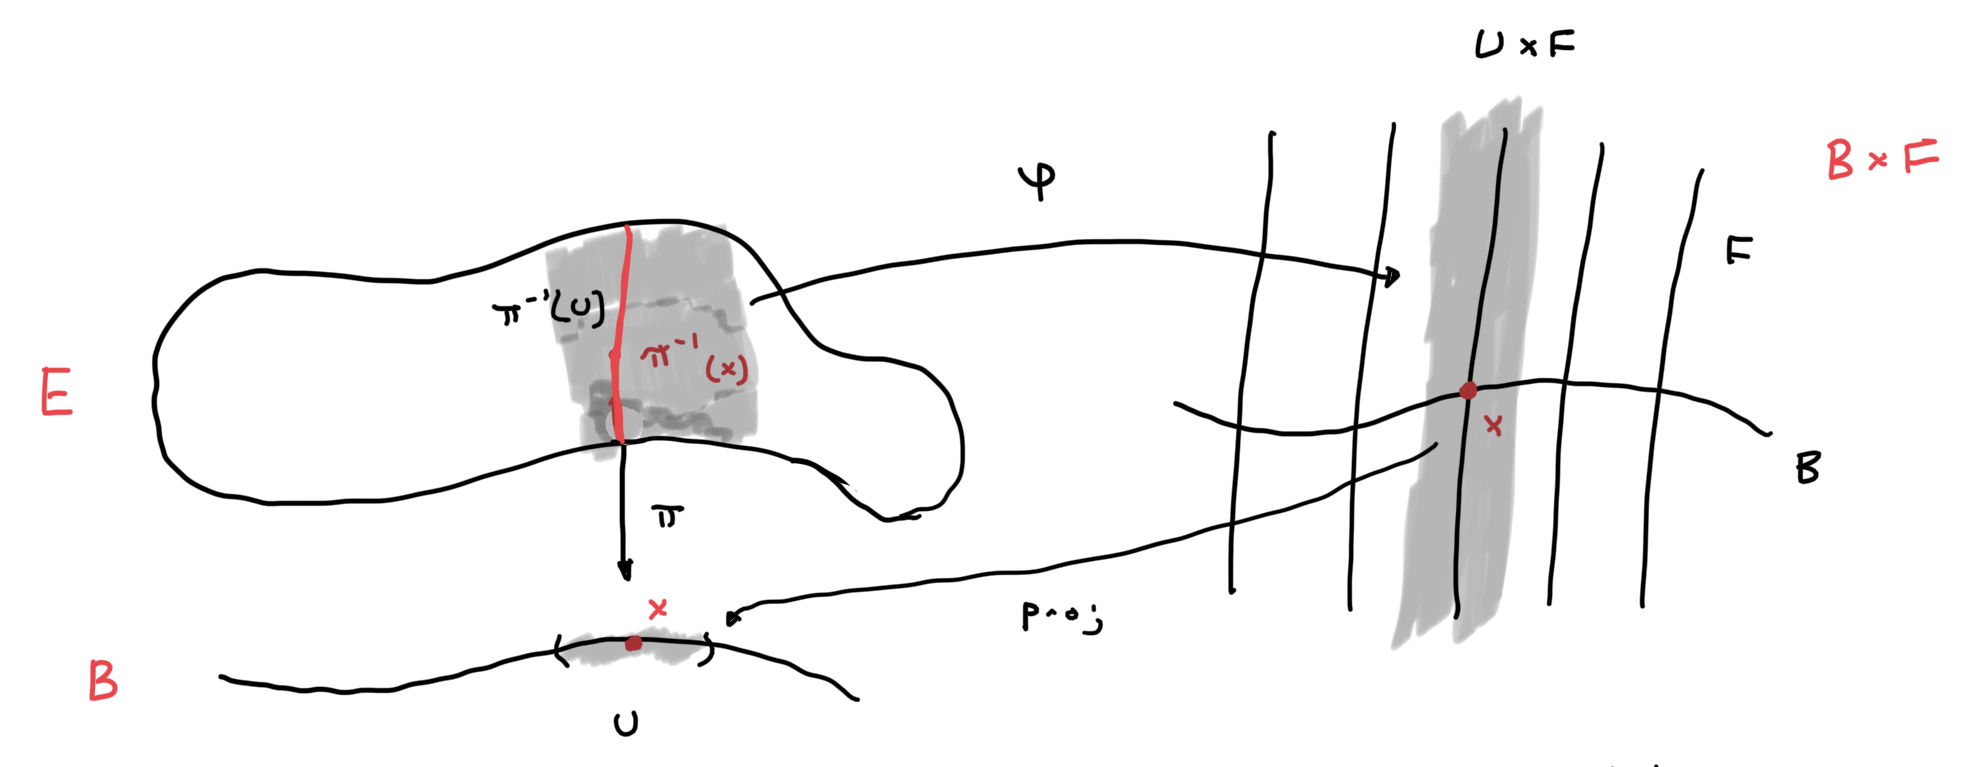
\includegraphics[width=\textwidth]{./assets/bundle4.jpeg}
\end{center}

\noindent Given some fibre bundle $(B, E, \pi, F)$, some collection of $\{U_i, \varphi_i\}$ which satisfy the local trivialization condition for each $x \in B$
is itself called a local trivialization (or, sometimes, an \emph{atlas}) for the fibre bundle. This is somewhat analogous to an atlas associated with a manifold: for a manifold,
we are giving information which reflects that a topological space is locally Euclidean, while here, we are giving information which reflects that the
total space is locally a product space of the base with the fibre!

To conclude this section, we present one more definition: we say that two bundles $(E, B, \pi, F)$ and $(E', B, \pi', F)$ with the same base space and model fibre are
\emph{isomorphic} if there exists a homeomorphism $h : E \rightarrow E'$ making the following diagram commute:
% https://q.uiver.app/#q=WzAsMyxbMCwwLCJFIl0sWzIsMCwiRSciXSxbMSwxLCJYIl0sWzAsMSwiaCJdLFsxLDIsIlxcbnUiXSxbMCwyLCJcXHBpIiwyXV0=
\[\begin{tikzcd}
E && {E'} \\
& X
\arrow["h", from=1-1, to=1-3]
\arrow["\pi'", from=1-3, to=2-2]
\arrow["\pi"', from=1-1, to=2-2]
\end{tikzcd}\]

\section{$G$-bundles and principal bundles}

\noindent Let $(E, B, \pi, F)$ be a fibre bundle. Let $\{U_i, \varphi_i\}$ be a local trivialization. Let $G$ be a topological group which acts continuously
on the model fibre $F$ (that is, the group action $G \times F \rightarrow F$ is a continuous map, where $G \times F$ and $F$ are given their usual topology).
We say that $\{U_i, \varphi_i\}$ is a \emph{$G$-atlas} of the fibre bundle if
each transition function $\varphi_j \circ \varphi_i^{-1} : U_i \cap U_j \times F \rightarrow U_i \cap U_j \times F$ can be written as
\begin{equation}
(\varphi_j \circ \varphi_i^{-1})(x, f) = (x, g_{ij}(x) \cdot f)
\end{equation}
where $g_{ij} : U_i \cap U_j \rightarrow G$ is a continuous function, and $g_{ij}(x) \cdot f$ is the group action of $g_{ij}(x)$ on $f \in F$. Said in English:
\newline

\noindent \emph{An atlas is a $G$-atlas if, whenever we have overlapping locally trivial regions in the base space, the corresponding mapping of fibres lying in the intersection
is dictated by the symmetries of some group.}
\newline

\noindent Said with pictures:

\begin{center}
  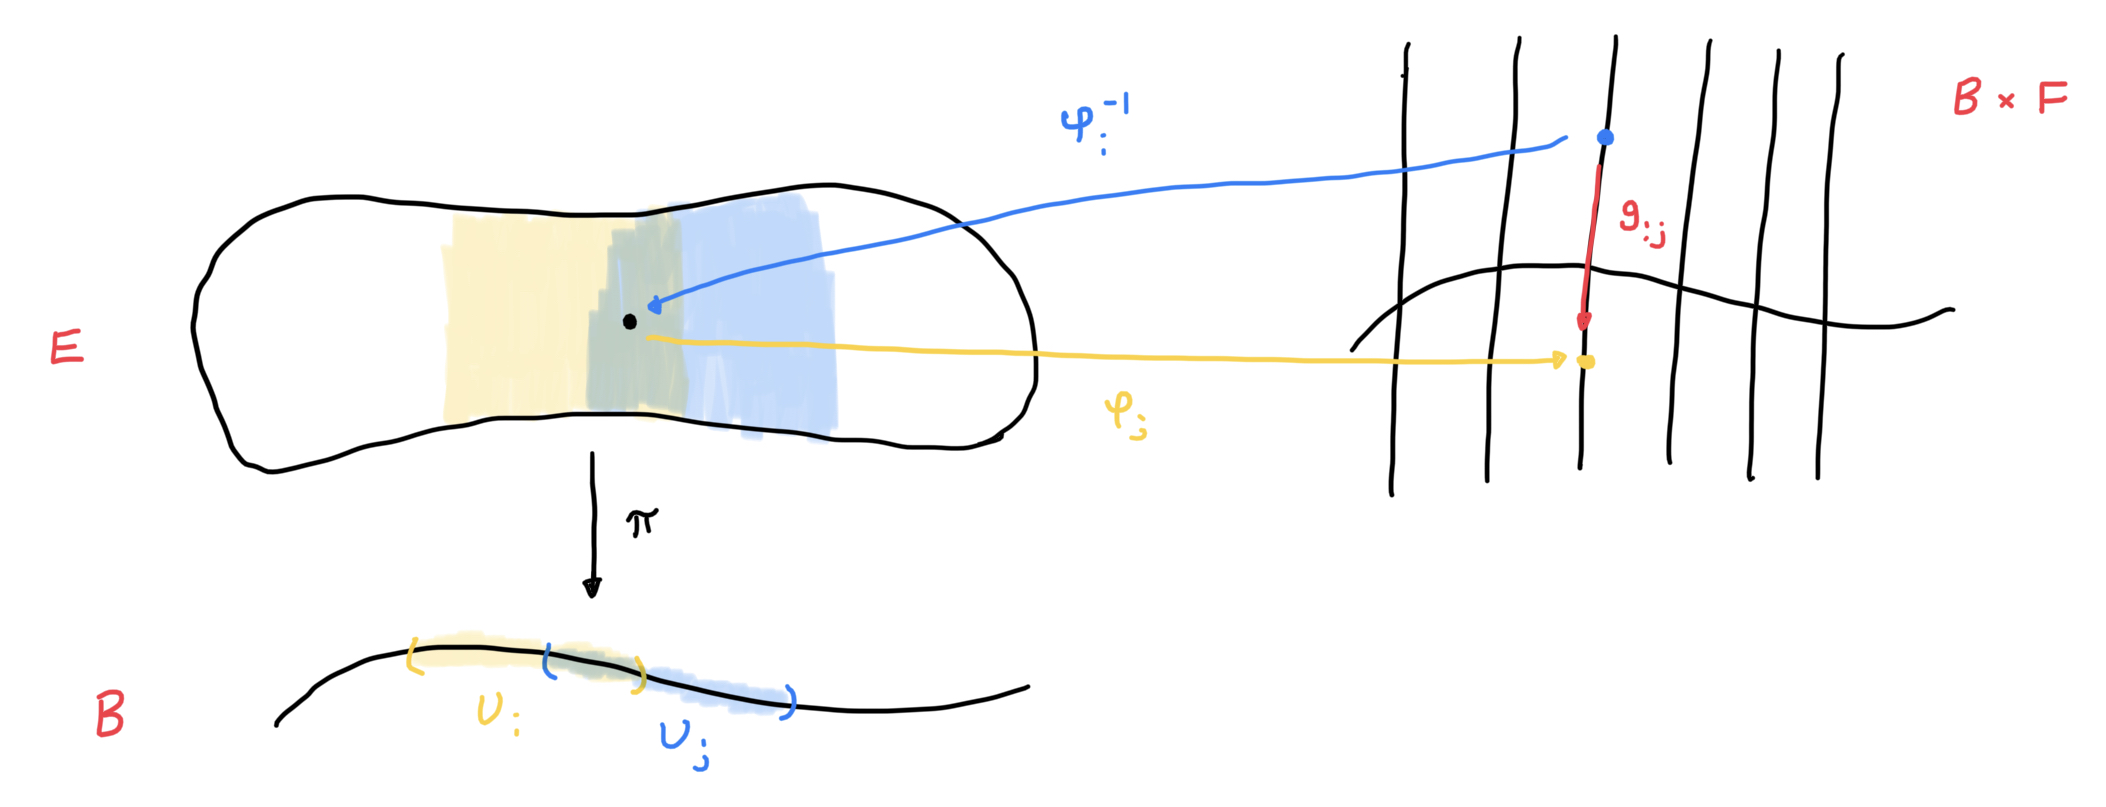
\includegraphics[width=\textwidth]{./assets/bundle3.jpeg}
\end{center}

\noindent We call a maximal $G$-atlas a \emph{$G$-structure} (similar to how a smooth structure is a maximal smooth atlas, in the theory of manifold). We call
a fibre bundle equipped with a given $G$-structure (if one exists) a \emph{$G$-bundle}. We call $G$ the \emph{structure group} associated with the $G$-bundle.
\newline

\begin{example}[Vector bundles]
The most basic example of a $G$-bundle is a vector bundle. To be specific, a vector bundle is a $G$-bundle in which the model fibre $F$ is
  either $\mathbb{R}^k$ or $\mathbb{C}^k$, and the structure group $G$ associated with transition functions is either $\text{GL}(k; \mathbb{R})$ or $\text{GL}(k; \mathbb{C})$,
  where the group action is simply multiplication of some element (a vector) of $\mathbb{F}^k$ (with $\mathbb{F} \in \{\mathbb{R}, \mathbb{C}\}$) by a matrix in $\text{GL}(k; \mathbb{F})$.
  \end{example}

    % Consider a fibre bundle $(B, E, \pi, \mathbb{F}^k)$ with local trivialization $\{(U_i, \varphi_i)\}$ ($\mathbb{F} \in \{\mathbb{R}, \mathbb{C}\}$), such that each fibre $\pi^{-1}(x)$ is a vector space,
    % with respect to some addition and scalar multiplication. Then the bundle if a vector bundle if and only if each map $\varphi_i : \pi^{-1}(x) \rightarrow \{x\} \times \mathbb{F}^k$
    % is an isomorphism of vector spaces, where addition and multiplication on $\{x\} \times \mathbb{F}^{k}$ is defined in the second factor.

\subsection{Adding more structure: principal bundles}

\noindent We have the following definition:

\begin{definition}[Principal bundle]
  We say that a $G$-bundle $\xi$ with structure group $G$ and corresponding $G$-structure $\mathcal{A}$ is a principal bundle if the action of $G$ on $F$
  is free and transitive. In particular:
  \begin{itemize}
  \item A group action $G \times X \rightarrow X$ is \emph{free} if $g \cdot x = x$, for some $g \in G$ and some $x \in X$ implies that $g = \text{id}$. In other words,
    \emph{there is no non-trivial group action which fixes a point of $X$}.
  \item A group action $G \times X \rightarrow X$ is \emph{transitive} if for any $x, y \in X$, we can find $g \in G$ such that $g \cdot x = y$. In other words,
    \emph{we can travel from any element in $X$ to any other element in $X$ via a group action}.
    \end{itemize}
\end{definition}

\noindent We call $F$ a \emph{principal homogeneous $G$-space} when $G$ acts in this way.

\begin{example}[$U(1)$ acting on $S^1$]
  Let us consider a very trivial example of a transitive and free group action: rotation of a circle. In particular, the obvious
  group action $U(1) \times S^1 \rightarrow S^1$ is given by complex multiplication $e^{i \theta} \cdot e^{i \varphi} = e^{i (\varphi + \theta)}$.
  Of course, if $e^{i \theta} \cdot e^{i \varphi} = e^{i \varphi}$, then $e^{i \theta} = 1$. In addition, given $\varphi$ and $\phi$, we have
  \begin{equation}
    e^{i (\phi - \varphi)} \cdot e^{i \varphi} = e^{i \phi}.
  \end{equation}
  Thus, the group action is free and transitive.
\end{example}

\noindent One of the most important example of principal bundles are so-called \emph{frame bundles}.

\begin{definition}[Frame bundle]
  Let $(B, E, \pi, \mathbb{F}^k)$ be a vector bundle. Let $\{U_i, \varphi_i\}$ be the corresponding $\text{GL}(k; \mathbb{F})$-structure.
  In this case, it is easy to see that each fibre $\pi^{-1}(x)$ is homeomorphic to $\{x\} \times \mathbb{F}^k$: the $k$-dimensional vector space over $\mathbb{F}$. In particular,
  given $x \in B$, there must be $U$ around $x$ and homeomorphism $\varphi : \pi^{-1}(U) \rightarrow U \times \mathbb{F}^k$ such that $\pi = \text{proj} \circ \varphi$. It follows that $\varphi(\pi^{-1}(x))$ must be sent by $\text{proj}$ to $x$, so
  must be sent into $\varphi(\pi^{-1}(x)) \subset \{x\} \times \mathbb{F}^k$. Moreover, since each $(x, f) \in \{x\} \times \mathbb{F}^k$ must be the target of some $u \in \pi^{-1}(U)$ via $\varphi$ (from surjectivity), we must have $\pi(u) = \text{proj}(x, f) = x$,
  so $u \in \pi^{-1}(x)$ and $\varphi(u) = (x, f) \in \varphi(\pi^{-1}(x))$, so $\{x\} \times \mathbb{F}^k \subset \varphi(\pi^{-1}(x))$. So, we have $\varphi(\pi^{-1}(x)) = \{x\} \times \mathbb{F}^k$, and we can simply restrict the homeomorphism $\varphi$ to the fibre.

  Let $[e_1, \dots, e_k]$ be an ordered basis for $\mathbb{F}_k$. We call the corresponding \emph{ordered} set of all pulled-back vectors, $[\varphi^{-1}(e_1), \dots, \varphi^{-1}(e_k)]$, a \emph{frame at $x$},
  where $\varphi : \pi^{-1}(U) \rightarrow U \times \mathbb{F}^k$ is an element of the local trivialization with $x \in U$. Note that the frame at $x$ is well-defined, independent of $\varphi$. In particular, if $\varphi$
  and $\varphi'$ are both elements of the local trivialization which have the fibre over $x$ in their domain, both will yield the same set of pulled-back ordered lists of vectors (this is straightforward to show, and is my
  assigned exercise to the class!).

  Let $F_x$ denote the set of all frames at $x$. We define the frame bundle as the disjoint union
  \begin{equation}
    F(E) = \bigsqcup_{x \in B} F_x \coloneqq \bigsqcup_{x \in B} \bigcup_{p \in F_x} (x, p)
  \end{equation}
  We can show that the frame bundle defines a valid principal bundle with structure group $\text{GL}(k; \mathbb{R})$ over base space $B$. Define
  \begin{equation}
    \widetilde{\pi} : F(E) \rightarrow B \ \ \ \ \text{where} \ \ \ \ \widetilde{\pi}(x, p) = x
  \end{equation}
  as the natural projection. By definition, for some $x \in B$, there exists some open $U$ around $x$ such that there is a homeomorphism $\varphi : \pi^{-1}(U) \rightarrow U \times \mathbb{F}^k$ such that $\pi = \text{proj} \circ \varphi$
  where $\pi : E \rightarrow B$ is the original bundle projection. Define
  \begin{equation}
    \widetilde{\varphi} : \widetilde{\pi}^{-1}(U) \rightarrow U \times \text{GL}(k; \mathbb{F}) \ \ \ \ \text{where} \ \ \ \ \widetilde{\varphi}(x, p) = (x, [\varphi(p_1), \dots, \varphi(p_k)])
  \end{equation}
  Such a map is well-defined, as $p \in F_x$, so it is of the form $[\varphi^{-1}(e_1), \dots, \varphi^{-1}(e_k)]$ for some ordered basis $[e_1, \dots, e_k]$. $\widetilde{\varphi}$ is a bijection: an element of the linear group,
  $[\varphi(p_1), \dots, \varphi(p_k)]$ is simply the change-of-basis-matrix sending the ordered standard basis to this new one. In addition, it is quite clear that $\widetilde{\pi} = \text{proj} \circ \widetilde{\varphi}$.

  We give $F(E)$ a topology which ensures that each $\widetilde{\varphi}$ is a homeomorphism, so $\{U_i, \widetilde{\varphi_i}\}$ is a local trivialization for the bundle. In particular,
  since each $\widetilde{\varphi}$ is a bijection, we simply say that $V \subset \widetilde{\pi}^{-1}(U)$ is open in $\widetilde{\pi}^{-1}(U)$ if and only if $\widetilde{\varphi}(V)$ is open in $U \times \text{GL}(k; \mathbb{F})$ (which
  itself already has a natural topology). We then give the whole space $F(E)$ the final topology induced by the inclusion maps $j : \widetilde{\pi}^{-1}(U_i) \xhookrightarrow{} F(E)$ of all the subspaces
  we have just topologized, for each $U_i$ in the local trivialization. Of course, the final topology is the finest topology on $F(E)$ for which each $j$ is continuous.
  Therefore, suppose $V \subset \widetilde{\pi}^{-1}(U) \subset F(E)$ is open in the subspace topology inherited from the final topology. Then $j^{-1}(V) = V$ is open in $\widetilde{\pi}^{-1}(U)$ with its induced topology, as each $j$ is continuous. It follows
  that $\widetilde{\varphi}(V)$ is open in $U \times \text{GL}(k; F)$, by definition of the induced topology. Moreover, if $V = \widetilde{\varphi}(\widetilde{\varphi}^{-1}(V)) \subset U \times \text{GL}(k; F)$ is open, then $\widetilde{\varphi}^{-1}(V)$ is open in $\widetilde{\pi}^{-1}(U)$ with the induced topology, so it must also be open in the final topology, as $j^{-1}(\widetilde{\pi}^{-1}(U))$ is open, and by definition, the final topology is the
  \emph{finest} topology in which the inclusions are continuous, so it will contain $\widetilde{\pi}^{-1}(U)$.

  It follows immediately that all the $\widetilde{\varphi}$ are homeomorphisms, and we immediately have defined a new bundle from the original vector bundle which
  we refer to as the \emph{frame bundle}. We can depict the creation of a frame bundle from a vector bundle diagrammatically:

\begin{center}
  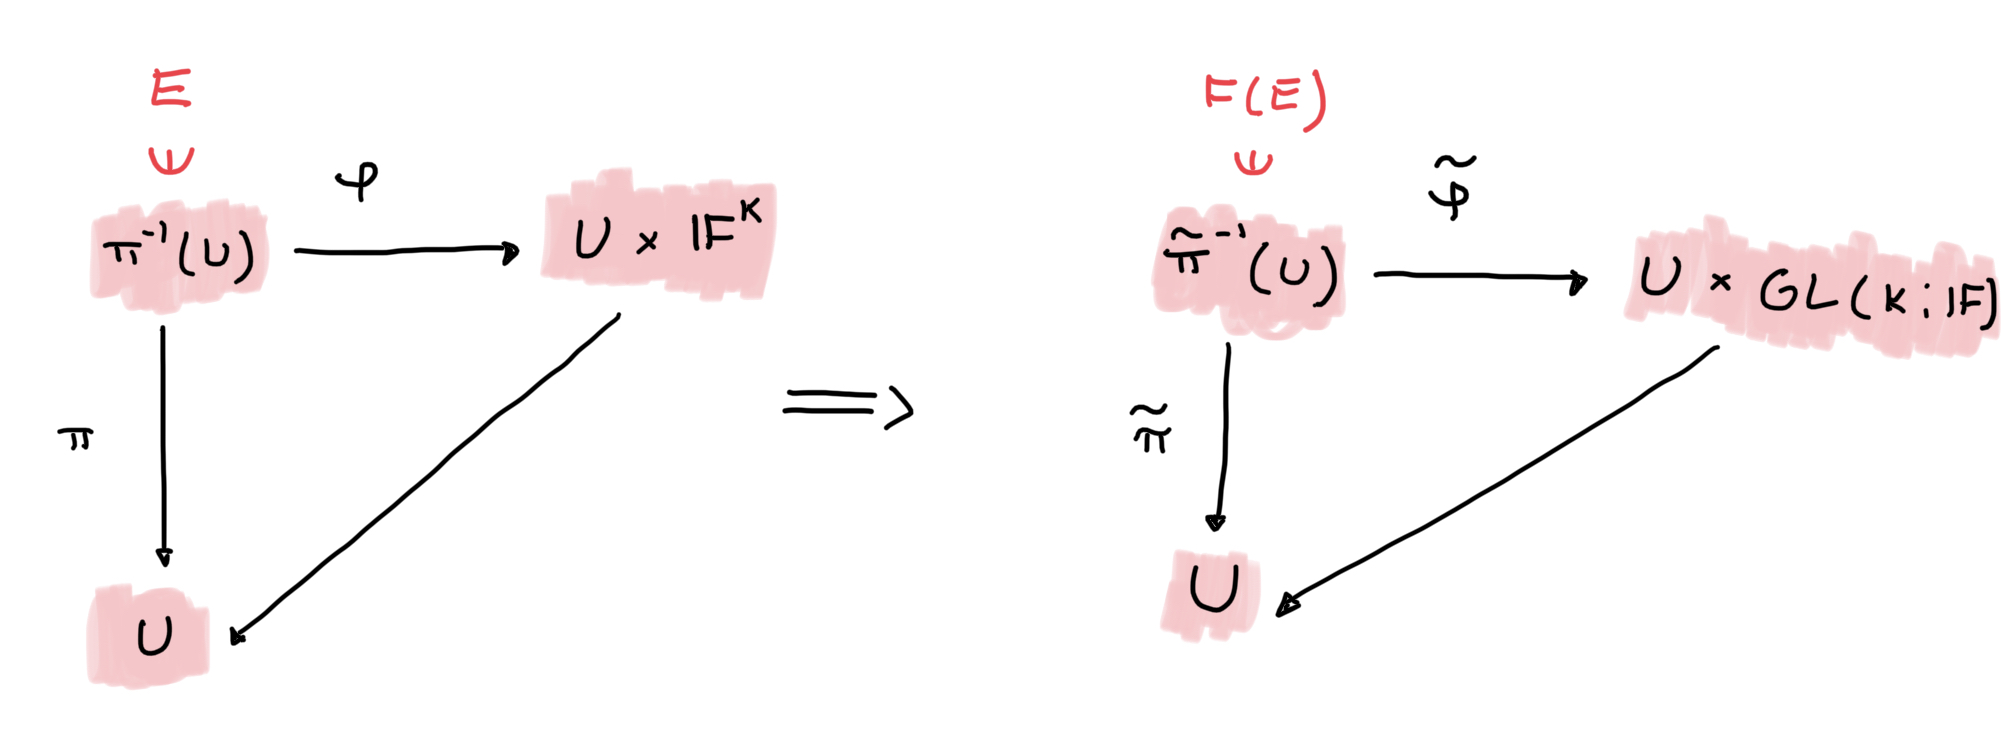
\includegraphics[width=\textwidth]{./assets/bundle5.jpeg}
\end{center}

\noindent In particular, note that the frame bundle is a vector bundle: the vector space is now $\text{GL}(k; \mathbb{F})$, and the group action on the fibres is precisely the same:
transition functions $\widetilde{\varphi}_i \circ \widetilde{\varphi}_j$ merely multiply an ordered basis by some element of $\text{GL}(k; \mathbb{F})$. The reason why our frame bundle is in fact
a \emph{principal bundle} as well is also easy to see:
\begin{itemize}
\item The group action is transitive, because, given two ordered bases $[e_1, \dots, e_k]$ and $[e_1', \dots, e_k']$, we can always find a change-of-basis matrix
  which goes from one basis to another, sending $e_k \mapsto e_k'$.
  \item The group action is free because if an element of $\text{GL}(k; \mathbb{F})$ sends an ordered basis to itself, we know by linearity that this matrix must simply be the identity.
  \end{itemize}

\end{definition}

\begin{example}[Frame bundle of a Riemannian manifold]
  An oriented Riemannian manifold $(M, g)$ has a natural frame bundle associated with it. In particular, let $TM$ be the tangent bundle associated with the manifold, which is itself a vector bundle.
  Let $\pi : TM \rightarrow M$ be the natural projection onto the basepoint of each of the tangent spaces $T_x M$.
  A local trivialization of this vector bundle is formed by the pushforwards of coordinate charts. In particular, suppose $x \in M$ with $\varphi : U \rightarrow \hat{U} \subset \mathbb{R}^n$
  a coordinate chart about $x$, then the differential
  $$d\varphi : \pi^{-1}(U) \rightarrow U \times \mathbb{R}^n \ \ \ \ \text{where} \ \ \ \ d\varphi(x, v) = (x, d_x \varphi(v))$$
  is the desired local homeomorphism (we ensure this is the case via a similar method as we topologized the frame bundle: we impose a natural topology on $TM$
  which forces each of these maps to be homeomorphisms). Note that $d_x \varphi : T_x M \rightarrow \mathbb{R}^n$ is the usual differential from the tangent space over $x$ to $\mathbb{R}^n$,
  which we know is an isomorphism, making $d\varphi$ an isomorphism as well.

  From this vector bundle, we can define a corresponding frame bundle.
In fact, because the tangent space has an associated metric, we are able to define special cases of the frame bundle: in particular, we can now speak of \emph{positively oriented orthonormal} ordered bases.
If we carry forward the same construction in the previous section, but replace ``ordered bases'' with ``positively oriented orthonormal bases'', we will arrive at the \emph{canonical manifold frame bundle}.
In this case, it is easy to see the structure group of the bundle will no longer be $\text{GL}(k; \mathbb{F})$, as such transformations may not send positively oriented orthonormal bases to other ones.
Instead, the structure group will be $\text{SO}(k; \mathbb{F})$: the subgroup which \emph{does} send positively oriented orthonormal bases to other positively oriented orthonormal bases.

To be more specific,
our transition functions $d\varphi_i \circ [d\varphi_j]^{-1}$ associated with the vector bundle, and thus those associated with the frame bundle, are precisely the Jacobians of the transition functions $\varphi_i \circ \varphi_j^{-1}$.
To see this, recall that if $\gamma'(0) \in T_x M$ (we use the tangent curve definition on tangent space), then $[d \varphi_j]^{-1}(x, r)$ for some $(x, r) \in U \times \mathbb{R}^n$ is an equivalence
class of tangent curves, $\gamma$, such that $(\varphi_j \circ \gamma)'(0) = (x, r)$. Thus, we will have
\begin{align}
  d \varphi_i(\gamma) = (\varphi_i \circ \gamma)'(0) = (\varphi_i \circ \varphi_j^{-1} \circ \varphi_j \circ \gamma)'(0) = D(\varphi_i \circ \varphi_j^{-1}) (\varphi_j \circ \gamma)'(0) = D(\varphi_i \circ \varphi_j^{-1}) \cdot (x, r)
\end{align}
where we simply use chain rule. Thus, $(x, r) \mapsto (x, D(\varphi_i \circ \varphi_j^{-1}) r)$ under the transition functions, so it follows that the corresponding group action is, once again, matrix multiplication.
However, when we restrict the frames themselves to be orthonormal
bases, and the transition functions are chosen in this way, it then follows immediately that the matrices whose multiplication induces the group action are in $\text{SL}(k; \mathbb{F})$, rather than the larger group $\text{GL}(k; \mathbb{F})$.
\end{example}

\section{Spin structure}

\noindent Having introduced all the relevant background material, we are now able to advance to the main construction that these notes attempt to introduce: spin structure.
To begin, suppose we have a $G$-bundle, $(B, E, \pi, F)$. We know that there is a group action of $G$ on the fibres, $G \times (\{x\} \times F) \mapsto \{x\} \times F$.
Via the local trivialization, this allows us to define an ``induced group action'' on the fibres $\pi^{-1}(x) \subset \pi^{-1}(U)$ in the total space:
% https://q.uiver.app/#q=WzAsNCxbMCwwLCJHIFxcdGltZXMgKFUgXFx0aW1lcyBGKSJdLFswLDIsIlVcXHRpbWVzIEYiXSxbMywyLCJcXHBpXnstMX0oVSkiXSxbMywwLCJHIFxcdGltZXMgXFxwaV57LTF9KFUpIl0sWzAsMSwiXFx0ZXh0e2dyb3VwIGFjdGlvbn0iLDJdLFsxLDIsIlxcdGV4dHtsb2NhbCBob21lb21vcnBoaXNtfSIsMCx7InN0eWxlIjp7InRhaWwiOnsibmFtZSI6ImFycm93aGVhZCJ9fX1dLFswLDMsIlxcdGV4dHtsb2NhbCBob21lb21vcnBoaXNtfSIsMix7InN0eWxlIjp7InRhaWwiOnsibmFtZSI6ImFycm93aGVhZCJ9fX1dLFszLDIsIlxcdGV4dHtpbmR1Y2VkIGBgZ3JvdXAgYWN0aW9uXCJ9IiwwLHsic3R5bGUiOnsiYm9keSI6eyJuYW1lIjoiZGFzaGVkIn19fV1d
\[\begin{tikzcd}
	          {G \times (U \times F)} &&& {G \times \pi^{-1}(U)} \\
	          \\
	            {U\times F} &&& {\pi^{-1}(U)}
	            \arrow["{\text{group action}}"', from=1-1, to=3-1]
	            \arrow["{\text{local homeomorphism}}", from=3-1, to=3-4]
	            \arrow["{\text{local homeomorphism}}"', from=1-4, to=1-1]
	            \arrow["{\text{induced ``group action"}}", dashed, from=1-4, to=3-4]
\end{tikzcd}\]
Thus, it makes sense to speak of ``the group action on fibres in the total space'', rather than having to always work in the model fibre. With this knowledge, we can present the main definitions:

\begin{definition}[Spin group]
  $\text{SO}(n)$ is the special orthogonal group consisting of all orthogonal $n \times n$ matrices, over some field, with unit determinant.
  This group is in fact a Lie group: it is a topological group that is also a manifold (as $\text{SO}(n)$ can be thought of as a subspace of $\mathbb{R}^{n^2}$,
  from which it is possible to see that a manifold structure in inherited). This manifold has a double cover, which is also a Lie group, called the \emph{spin group},
  which we denote by $\text{Spin}(n)$.
  \end{definition}

\begin{definition}[Spin structure]
  Suppose we are provided with an principal $\text{SO}(n)$-bundle $(B, E, \pi, F)$ (so, this is a $G$-bundle with structure group $\text{SO}(n)$ such that the group action is free and transitive) with
  base space $B$.
  We say that a \emph{spin structure} is a principal $\text{Spin}(n)$-bundle $(B, \widetilde{E}, \widetilde{\pi}, \widetilde{F})$ over the same base space $B$, along with a map $f$, such that the following diagram commutes:
  % https://q.uiver.app/#q=WzAsNSxbMCwwLCJcXHRleHR7U3Bpbn0obikgXFx0aW1lcyBcXHdpZGV0aWxkZXtFfSJdLFszLDAsIlxcd2lkZXRpbGRle0V9Il0sWzAsMiwiXFx0ZXh0e1NPfShuKSBcXHRpbWVzIEUiXSxbMywyLCJFIl0sWzUsMSwiQiJdLFswLDEsIlxcdGV4dHtpbmR1Y2VkIGdyb3VwIGFjdGlvbn0iXSxbMCwyLCJcXHRleHR7ZG91YmxlIGNvdmVyfSBcXHRpbWVzIGYiLDJdLFsyLDMsIlxcdGV4dHtpbmR1Y2VkIGdyb3VwIGFjdGlvbn0iXSxbMSwzLCJmIl0sWzEsNCwiXFx3aWRldGlsZGV7XFxwaX0iXSxbMyw0LCJcXHBpIiwyXV0=
  \[\begin{tikzcd}
	          {\text{Spin}(n) \times \widetilde{E}} &&& {\widetilde{E}} \\
	          &&&&& B \\
	          {\text{SO}(n) \times E} &&& E
	          \arrow["{\text{induced group action}}", from=1-1, to=1-4]
	          \arrow["{\text{double cover} \times f}"', from=1-1, to=3-1]
	          \arrow["{\text{induced group action}}", from=3-1, to=3-4]
	          \arrow["f", from=1-4, to=3-4]
	          \arrow["{\widetilde{\pi}}", from=1-4, to=2-6]
	          \arrow["\pi"', from=3-4, to=2-6]
  \end{tikzcd}\]
\end{definition}

\noindent If we are provided with a Riemannian manifold, in order to construct a spin structure, we need a principal $\text{SO}(n)$-bundle. Luckily, there is a natural choice
for such a bundle, the \emph{\textbf{canonical manifold frame bundle}}, which we constructed earlier.

\begin{definition}[Canonical spin structure on a manifold]
  A canonical spin structure for a given, oriented Riemannian manifold is precisely a principal $\text{Spin}(n)$-bundle which ``covers'' (in the sense of the above definition),
  the canonical manifold frame bundle, which is of course a principal $\text{SO}(n)$-bundle. Note that the spin structure for a manifold is generally, \emph{non-unique}.
  \end{definition}

\end{document}
